\subsection{Context}
The database exists to store the images used by the neural network, including training data, and data collected at runtime for future training and testing. 
Images will generally be added one at a time during runtime, but during testing and development the capability to add several, potentially hundreds of images per transaction. 

\subsection{Dependancies} 
The database will not depend on any other subsystem for opperation.

\subsection{Structure}
Making use of SQLite, the database itself will consist of a single file, alongside a folder containing the named image files. 
The database will consist of several tables, one for the training, one for verification, and one for images collected during runtime. 
The training table will consist of the following columns: index (integer), image address (String), actual type(boolean). 

\begin{figure}[h]
\caption{testing database example}
\centering
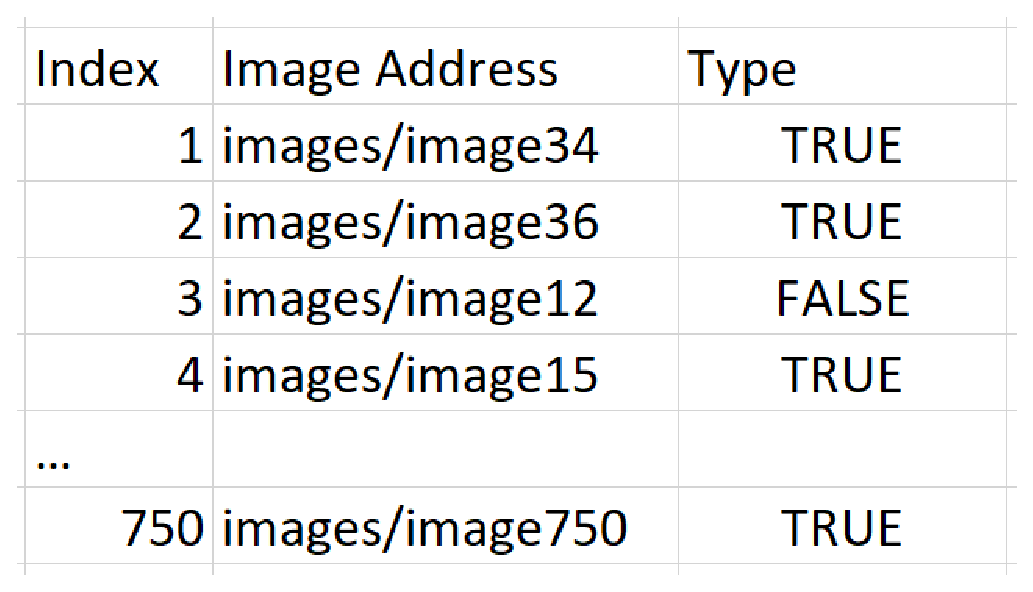
\includegraphics[height=4cm]{testingdb}
\end{figure}

The verification table will consist of the same columns with the addition of a flag column to indicate that during verification, the neural net missclassified the image in the entry. 

\begin{figure}[h]
\caption{verification database example}
\centering
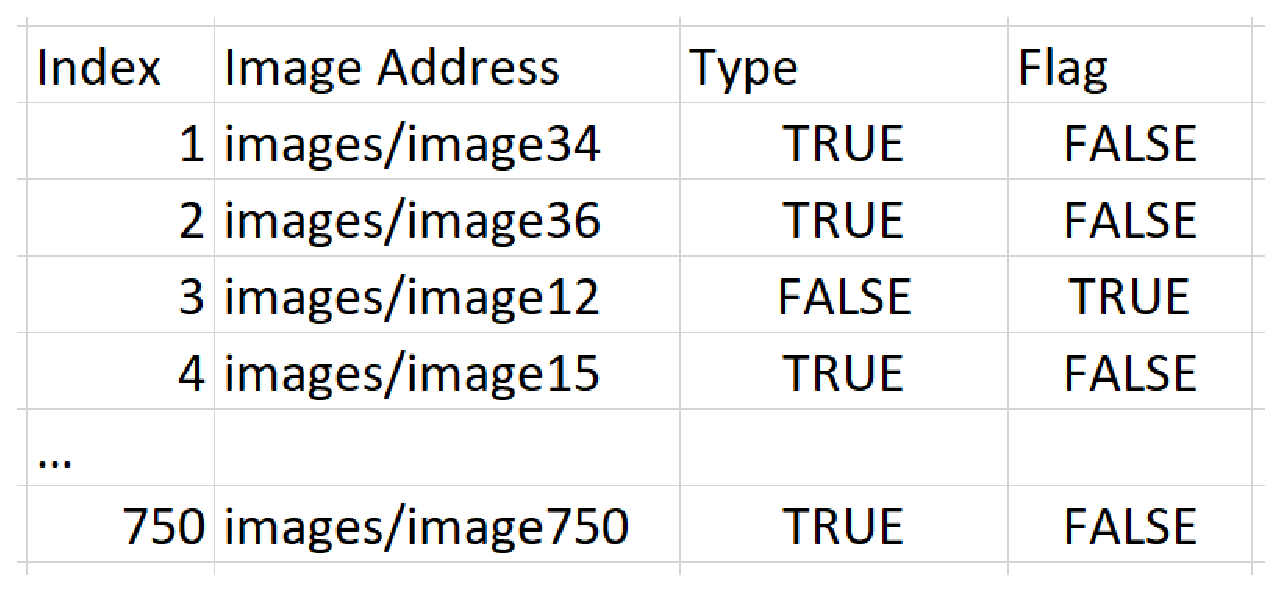
\includegraphics[height=4cm]{verificationdb}
\end{figure}


Finally the runtime table will consist of an index (integer), image address (String), and guess(boolean).

\begin{figure}[h]
\caption{runtime database example}
\centering
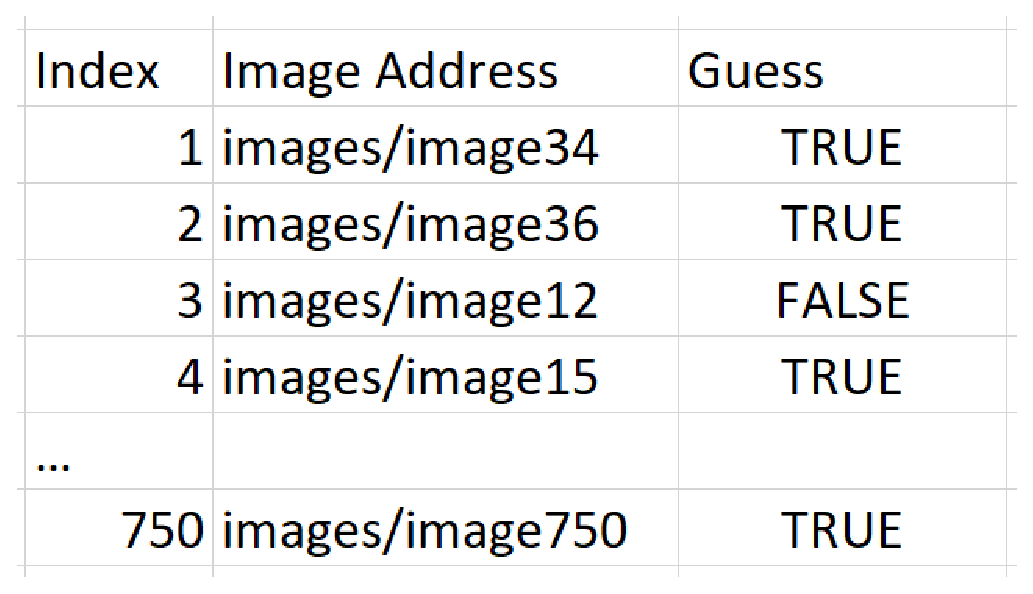
\includegraphics[height=4cm]{runtimedb}
\end{figure}

Each of these tables will share a database file, and a folder to store images in.
While not in use, this foder could be compressed into a tar archive, but would be uncompressed before runtime or during startup.




\subsection{Logical}

The database will be coded to support the following functions:

\begin{minted}{Python}

#returns the image address associated with the given the db index.
entry getImage(index, table);

#returns the image addresses associated with the given index range.
getImages(start, end, table);

#adds [num] entries to the db table.
void addImages(entries, int num, table);

#performs the given query, and returns an array containing the results.
query(query);

\end{minted}

The getImage, and getImages functions are designed to allow easy querying of images iteratively during neural network training. In such cases, we only care that each data point gets used, and filtering results based on type or guess is unlikely to be necessary.
The addImages function allows the system to add add the seed images collected during runtime to the database.
The query function allows us to move entrys to different table in order to increase the size of the training or verification data sets. 

\subsection{Interaction}

The database will interact with other subsystems by receiveing and servicing requests to access data in the database. During training, this will be returning entries from the training and verification data sets. At runtime, the system will present images to save via the addimages function. Each iteration, developers will utilize the query function to perform less typical opperations, including migrating runtime data into the training and verification tables.

\subsection{Resources}

The database will require little RAM, but will require its own drive in order to support storing a large number of images. We estimate that drive size will be close to 10 GB, but depending on the size of the training dataset, additional or less memory may be necessary.


